\section{Достоверность партонной модели при ПэВ-энергиях}
Актуальность исследования достоверности сечений взаимодействия нейтрино с нуклоном при энергиях порядка ПэВ связана с ограниченной областью  $(x, Q^2)$ экспериментально изученных партонных распределений. На рис. (\ref{fig:xQ2_PDG}) приведена исследованная область в экспериментах на коллайдерах:   БАК (LHC), Теватрон, HERA, а также в экспериментах с неподвижной мишенью.  
\begin{figure}[!h]
\centering
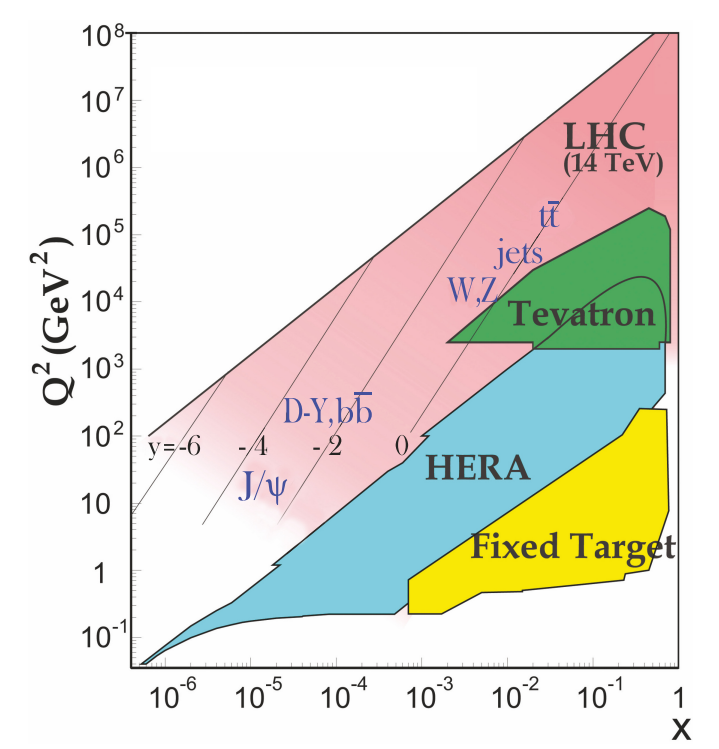
\includegraphics[width=\linewidth]{images/NuProp/reald}
\caption{Кинематические области в $x$ и $Q^2$, исследованные в экспериментах с неподвижной мишенью и на коллайдерах. Рисунок из \cite{ParticleDataGroup:2024cfk}.}
\label{fig:xQ2_PDG}
\end{figure}
Область малых $x\lesssim 10^{-6}$ исследованна довольно слабо. Между тем, с ростом энергии взаимодействия нейтрино, вклад именно малых $x$ в сечение взаимодействия становится доминирующим. Выход в неисследованную область требует использования экстраполяции. 


\subsection{Полное сечение и его вариация от параметризации}
На рис.~\ref{fig:xsec_total} показана зависимость полного сечения взаимодействия мюонного нейтрино на нуклоне от энергии для различных партонных распределений. Также, приведена вариация полного сечения, связанная с использовании разных наборов партонных распределений.

\begin{figure}[!h]
\centering
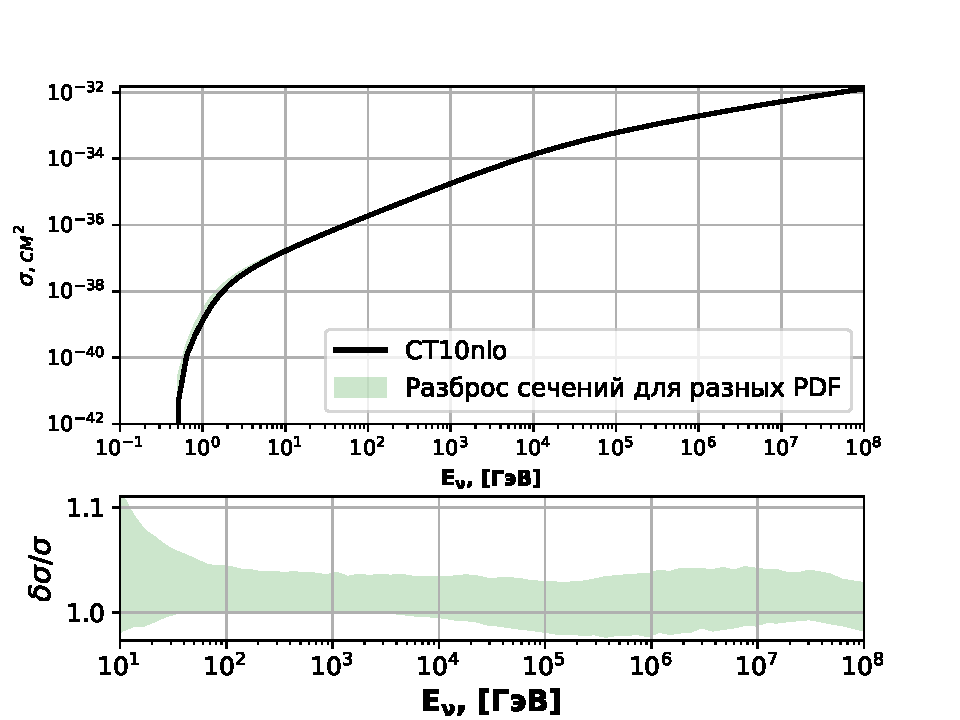
\includegraphics[width=\linewidth]{images/NuProp/xs_vs_enu.pdf}
\caption{Полные сечения взаимодействия мюонного нейтрино на нуклоне в зависимости от энергии $E_\nu$ для партонных распределений \texttt{CT10nlo}. Полоса отвечает вариации полного сечения при использовании других наборов партонных распределений (\texttt{CT18ZNNLO}, \texttt{nCTEQ15}, \texttt{TUJU19\_nlo}).} 
\label{fig:xsec_total}
\end{figure}

\subsection{Вклад экспериментально недоступной области}

\begin{equation}
CDF(x) = \int\limits_{x}^1\frac{d\sigma(E,x')}{dx'}dx'
\end{equation}


Чтобы количественно оценить вклад неизведанной области в полное сечение взаимодействия нейтрино с нуклоном  определим отношение: 
 \begin{equation}
     F_{\sigma}(x_\text{min},Q^2_\text{min}) = \frac{1}{\sigma(E_{\nu})}\int\limits_{x_\text{min}}^1dx\int\limits_{Q^2_\text{min}}^{Q^2_\text{max}}dQ^2\frac{d^2\sigma}{dxdQ^2}.
 \end{equation}
На рисунках (\ref{Pp3})-(\ref{Pp8}) приведена $F_{\sigma}(x_\text{min},Q^2_\text{min})$ в зависимости от $x_\text{min}$ и $Q^2_\text{min}$ для трёх примеров энергии нейтрино: 1 ТэВ, 1 ПэВ, 100 ПэВ. 
 
Линии на рисунках указывают области, где сечения насыщаются до определенного уровня: $10\%$, $50\%$, $90\%$. Серая штрихованная область качественно отмечает экспериментально доступную область, приведённую на рис.~\ref{fig:xQ2_PDG}.

Видно, что область насыщения сечений частично выходит из области экспериментальных данных. При высоких энергиях  - это область в диапазоне $10^2\le Q^2\le10^{4.5} $ и $10^{-5}\le x \le 10^{-9}$.  
\begin{figure}[!h]
\centering
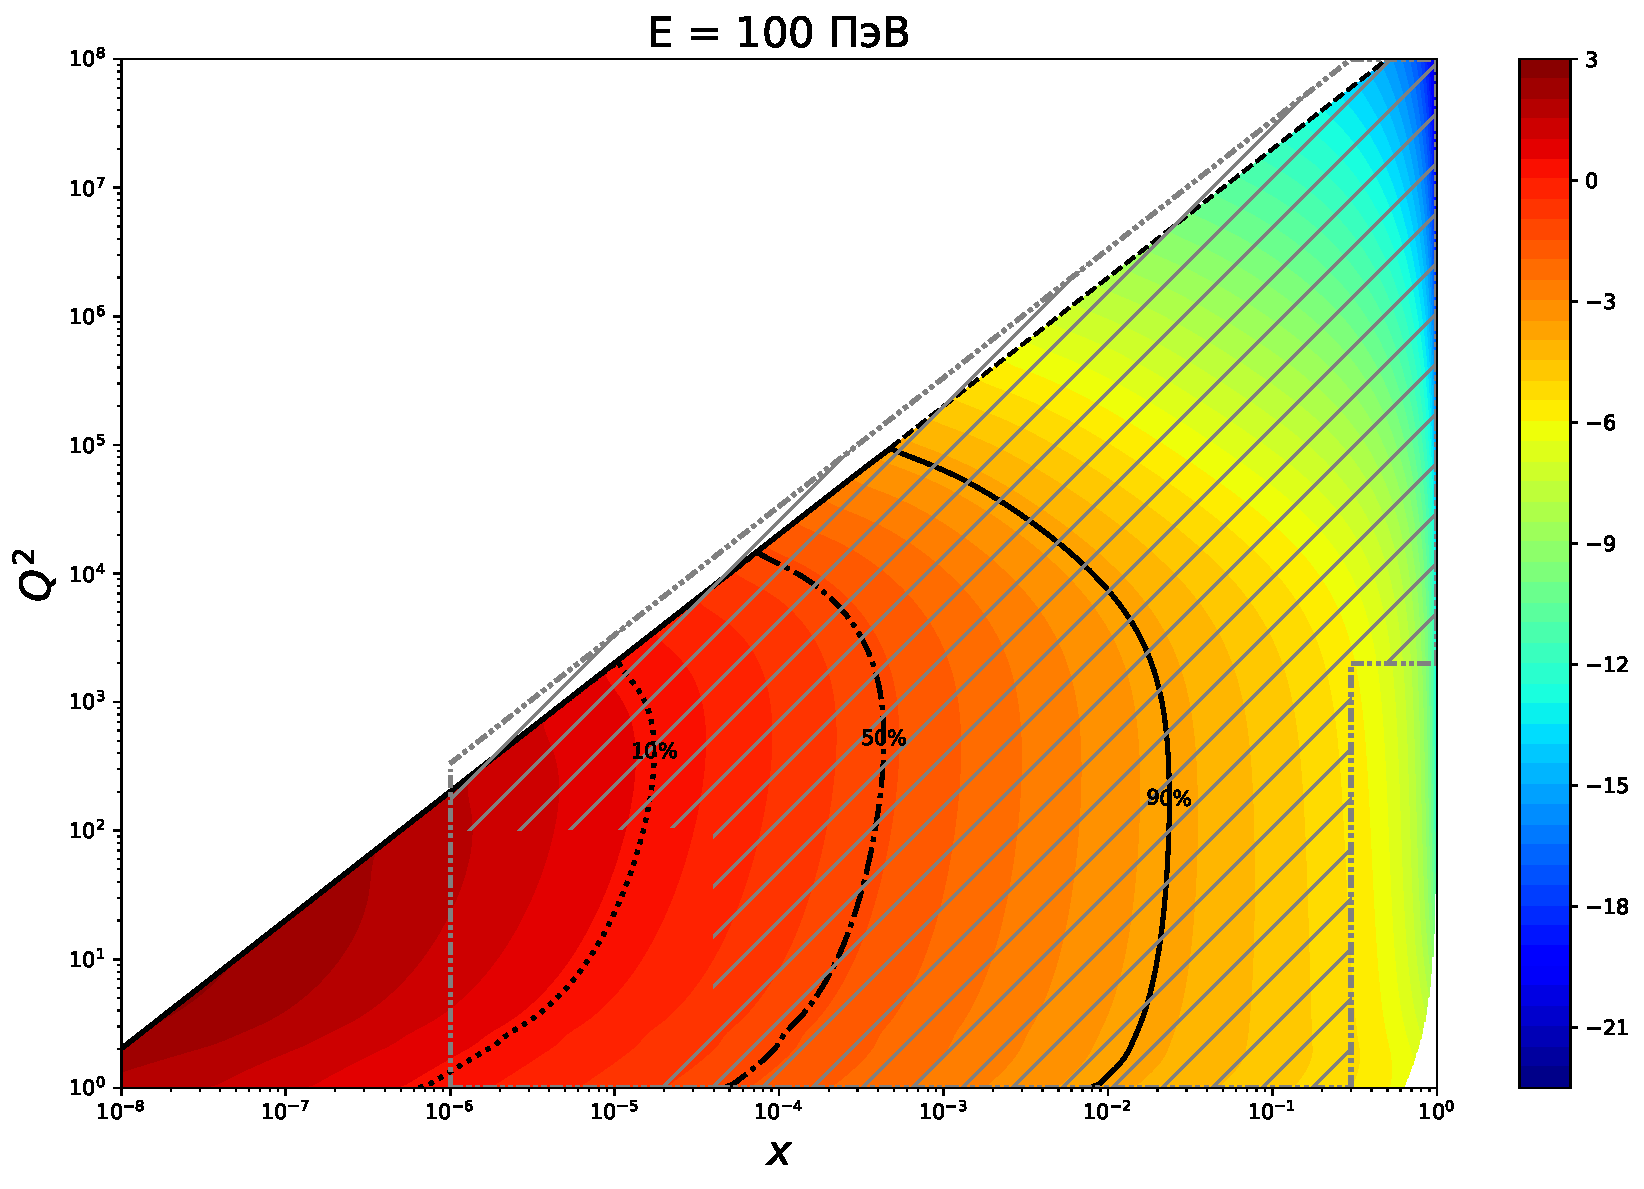
\includegraphics[width=0.97\linewidth]{images/NuProp/cdfxq2_cc_proton_CT18ZNNLO_14_100000000.pdf}
\caption{Зависимость кумулятивного нормированного сечения $F_{\sigma}(x,Q^2)$ в зависимости от переменной Бъеркена $x$ и переменной $Q^2$ для энергии нейтрино $E_{\nu} = 100$ PeV для модели партонных распределений CTEQ15\cite{ncteq15}.}
\label{Pp8}
\end{figure}
